\section{Failures at Scale}
In this section we discuss how and why knowledge markets may fail at scale. We first empirically examine diseconomies of scale (Section 8.1), then analyze the effects of scale on market health (Section 8.2), and finally study market stability under user perturbation (Section 8.3).

\subsection{Diseconomies of Scale}
First, we examine disceconomies of scale---the ratio of answers to questions declining with the increase in number of users. The opposite of diseconomies is economies---the ratio of answers to questions increasing with the increase in number of users. The concept of diseconomies is important because the decrease in answer to question ratio implies the increase in the gap between market supply (answer) and demand (question). In fact, if the ratio falls below 1.0, the gap becomes critical---guaranteeing there will be some questions with no answers. We observe disceconomies of scale in most Stack Exchange markets.

Figure~\ref{fig:diseconomy} shows three examples of diseconomies and economies (the reverse of diseconomies): \texttt{cstheory}, \texttt{puzzling} and \texttt{superuser}. Among the three markets, \texttt{superuser} shows strong diseconomies of scale---if the number of users increases by 100\%, the answer to question ratio declines by a factor of x.x. The other two markets are counter examples, where \texttt{cstheory} shows strong economies of scale---if the number of users increases by 100\%, the answer to question ratio increases by a factor of x.x; and \texttt{puzzling} shows weak economies of scale---if the number of users increases by 100\%, the answer to question ratio increases by a factor of x.x. Note that most markets, especially the ones with 500+ monthly active participants, exhibit diseconomies of scale similar to \texttt{superuser}. The markets that exhibit economies of scale are rare; we found four such markets in Stack Exchange: \texttt{cstheory}, \texttt{expressionengine}, \texttt{softwareengineering}, \texttt{hardwarerecs}.

\begin{figure}[hbt]
\centering
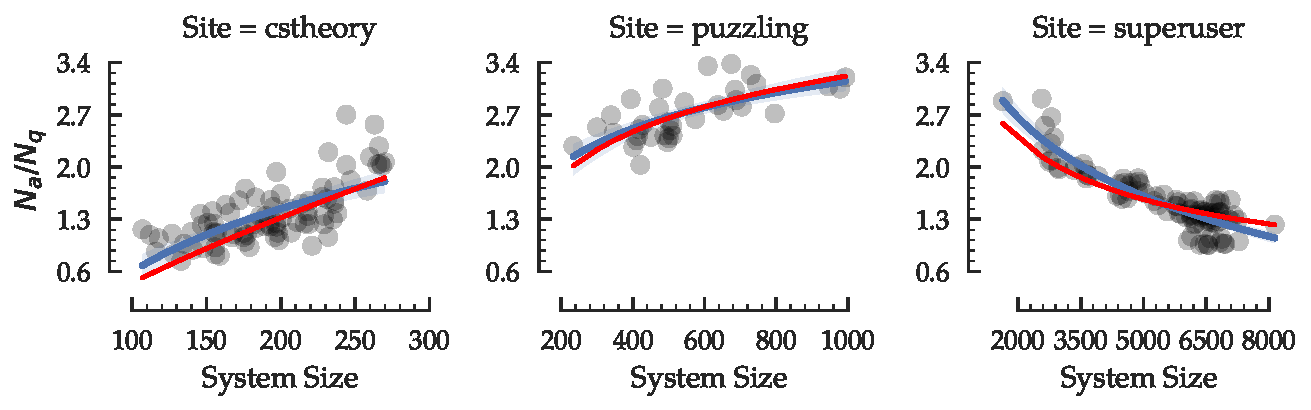
\includegraphics[scale=0.38]{Figures/Size_vs_Diseconomy.pdf}
\caption{Economies and disecnomies of scale: \texttt{cstheory} (strong economies), \texttt{puzzling} (weak economies) and \texttt{superuser} (strong diseconomies). Most markets exhibit diseconomies of scale similar to \texttt{superuser}.}
\label{fig:diseconomy}
\end{figure}

The Cobb-Douglas curves well fit the empirical trends of economies and diseconomies. We derive these curves by dividing the answer models by the corresponding question models. We get similar curves via log regression as shown in Figure~\ref{{fig:diseconomy}}. Between the two model types, the Cobb-Douglas models provide better explanation.

The Cobb-Douglas models well explain the economies and disceconomies of scale. Based on the models, the primary cause of disceconomies is the difference between the diminishing returns of questions and answers for users. In other words, for user input, the marginal question output is higher compared to marginal answer output, i.e., an average user is likely to ask more questions and provide few answers. This causes the ratio of answers to questions to decline with the increase in number of users.

\subsection{Analyzing Health}
Next, we examine the disadvantage of scale through three health metrics: percentage of questions with at least one answer, percentage of questions with accepted answer, and average number of upvotes per content. The first two metrics capture the utility received by askers, whereas the third metric captures the utility received by any active user. The decline in answer to question ratio may cause decline in the first two health metrics. In fact, if the ratio falls below 1.0, it guarantees the decline of these metrics. Figure x shows the disadvantage of scale through health metrics for three markets: academia, android and tex. We observe that all three health metrics decline at scale. \textcolor{blue}{Figure: Plot to show the decline of health metrics at scale.}

We cluster the markets based on model parameters and examine their health. In particular, we use kmeans clustering with silhouette analysis to determine two clusters. Figure x shows the clusters in a 3d space, reduced via Isomap reduction. Figure y shows the health summary for the two clusters. There exists a clear gap between the health of the two clusters. The first group is somewhat more robust to scale, whereas the second group is vulnerable at scale.

\begin{figure}[hbt]
\centering
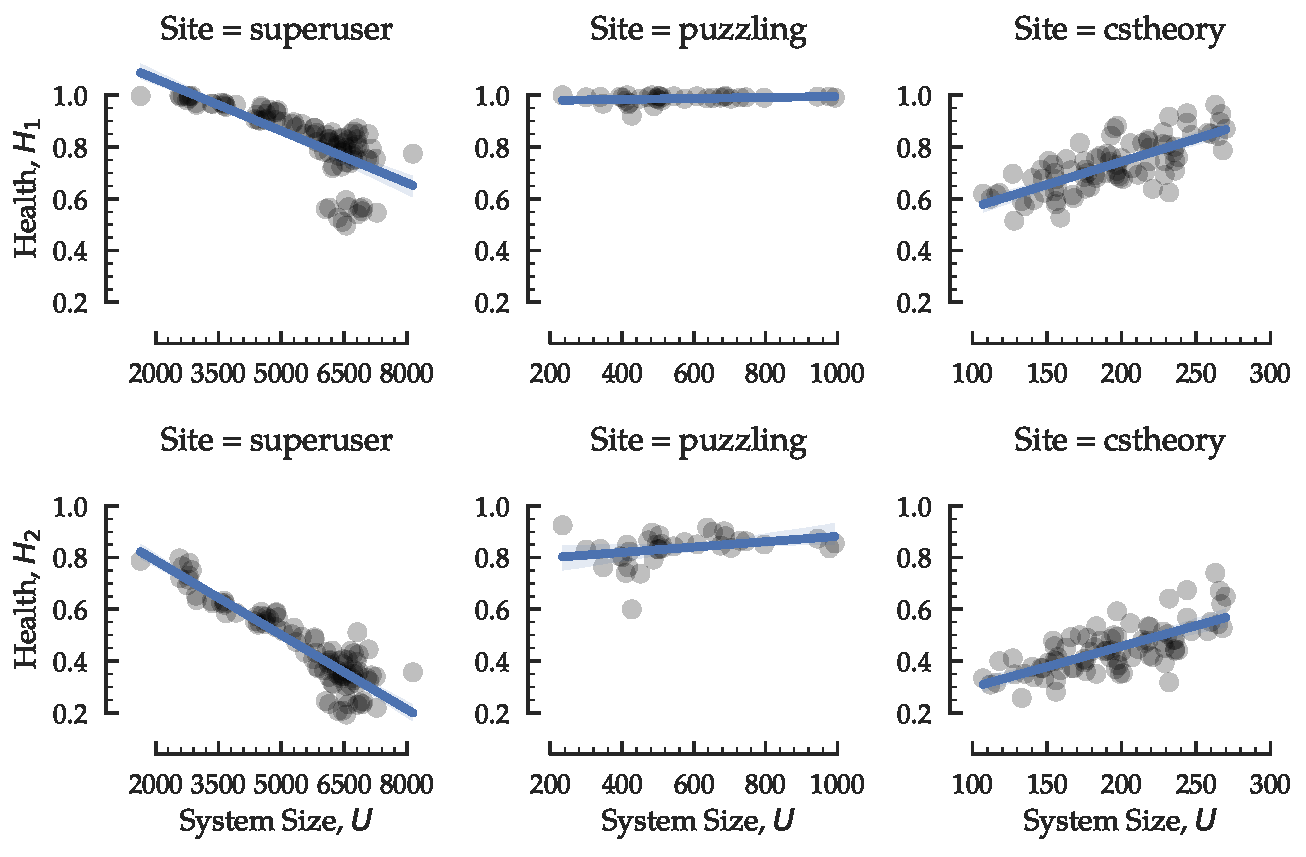
\includegraphics[scale=0.38]{Figures/Size_vs_Health.pdf}
\caption{Long caption}
\label{fig:health}
\end{figure}

\subsection{Effects on Stability}
Now, we study market stability under user perturbation. We concentrate on how many users
As the stability of knowledge markets depend on user participation, we investigate the effect of scale on stability. \textcolor{blue}{Yet to add details. Figure: Plot to show stability as a function of economic parameters/size/etc.}

\begin{figure}[hbt]
\centering
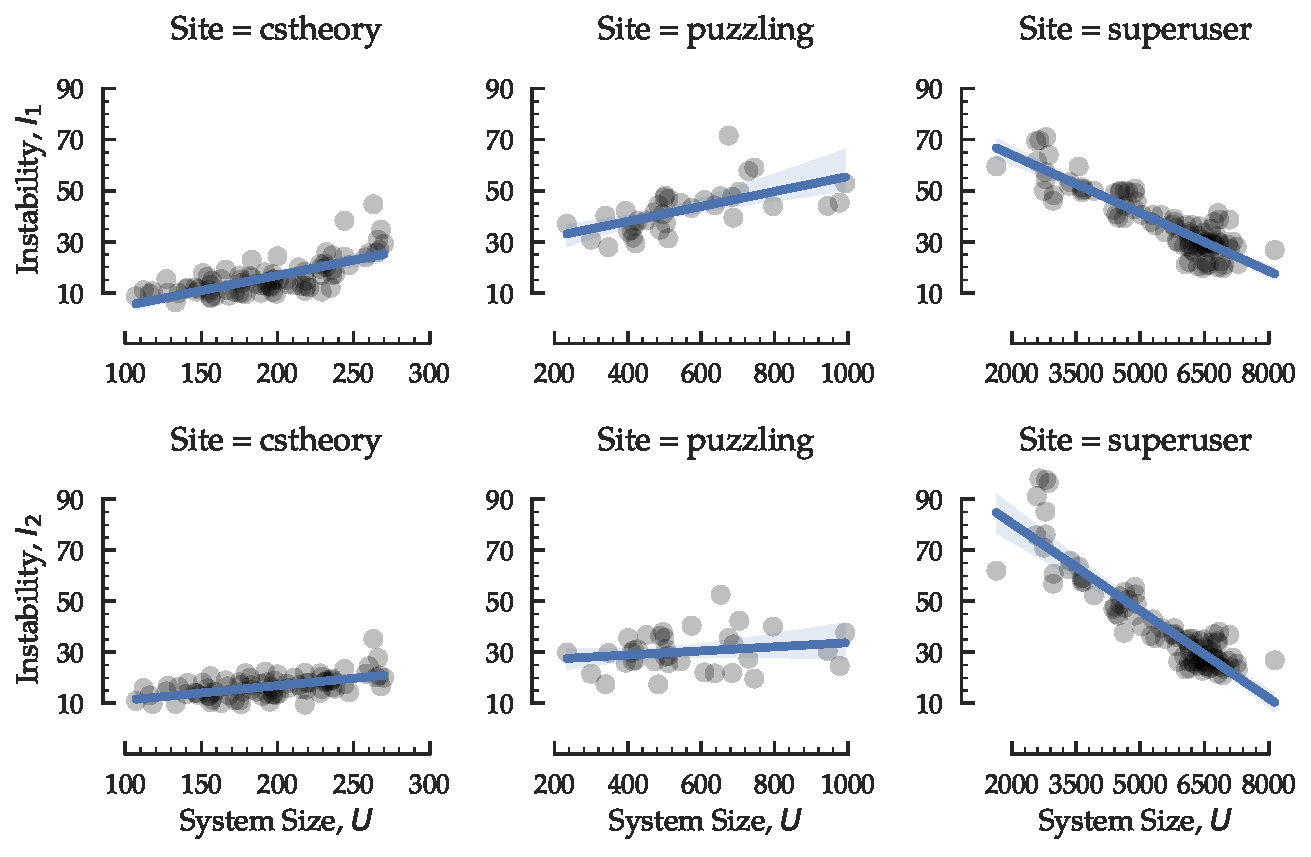
\includegraphics[scale=0.38]{Figures/Size_vs_Instability.pdf}
\caption{Long caption}
\label{fig:stability}
\end{figure}


